%=== CHAPTER ONE (1) ===
%=== INTRODUCTION ===
\setlength{\columnsep}{1cm}
\section{Introduction}
\begin{spacing}{2.0}

Chess is a game of strategy and skill that has captivated players and spectators for centuries. As the popularity of chess continues to grow, there is a growing interest in understanding the characteristics and abilities of individual chess players. The ability to identify chess players based on their playing style and patterns can provide valuable insights into player profiling, performance analysis, and talent identification. However, manual identification of chess players is a laborious and subjective task, often limited by human biases and errors. Recent advancements in machine learning, particularly neural networks, offer promising opportunities to automate the identification process and extract meaningful patterns from large volumes of chess data.

This paper aims to explore the identification of chess players through the application of neural networks. The research is motivated by the desire to develop an automated system capable of accurately recognizing individual chess players based on their unique playing styles and strategies. By leveraging neural networks, this study intends to enhance our understanding of player characteristics and facilitate practical applications within the chess community.

Positioning this research within the field of machine learning, chess analysis, and player profiling, the investigation will follow the research onion framework as shown in Figure~\ref{fig:Onion}. This framework will guide the investigation into the identification of chess players through neural networks. Adopting a positivist research philosophy, the study aims to uncover objective and quantifiable patterns in player identification. The research approach is deductive, involving the formulation of hypotheses that will be tested using collected data. Furthermore, a mixed method approach combining grounded theory, archival research, and experimental strategies is employed to provide a comprehensive understanding of player identification. The time horizon for this study is cross-sectional, focusing on a snapshot of player identification patterns. Data collection involves the extraction of historical chess game data from archival sources. Data analysis techniques include qualitative coding, statistical analysis, and training neural networks to recognize patterns in chess player identification. By integrating these various elements, this research aims to contribute to the field's understanding of identifying chess players through neural networks.

The background to this research theme lies in the limitations of manual identification methods, which are time-consuming, subjective, and prone to human biases and errors. Previous attempts to automate player identification have relied on rule-based systems or statistical techniques, which often fail to capture the complex patterns and nuances of individual playing styles. The advancements in machine learning and neural networks provide a compelling opportunity to overcome these limitations and offer a more accurate and objective means of identifying chess players. The most recent and best attempt so far was by Mcllroy-young et al, whom managed to obtain promising results even when lacking information \cite{stylometryChess}.

The hypothesis for this research posits that by training neural networks on extensive datasets of chess games, it is possible to develop an automated system that accurately identifies individual chess players based on their unique playing styles and strategies.

The research aim is to explore the application of neural networks for the identification of chess players, with the purpose of developing an automated system capable of effectively recognizing and differentiating chess players based on their playing patterns and strategies. The intended outcomes include enhancing our understanding of player characteristics, contributing to player profiling and analysis, and enabling practical applications such as player rankings, talent identification, and personalized coaching within the chess community.

\begin{figure}[ht]
\centering
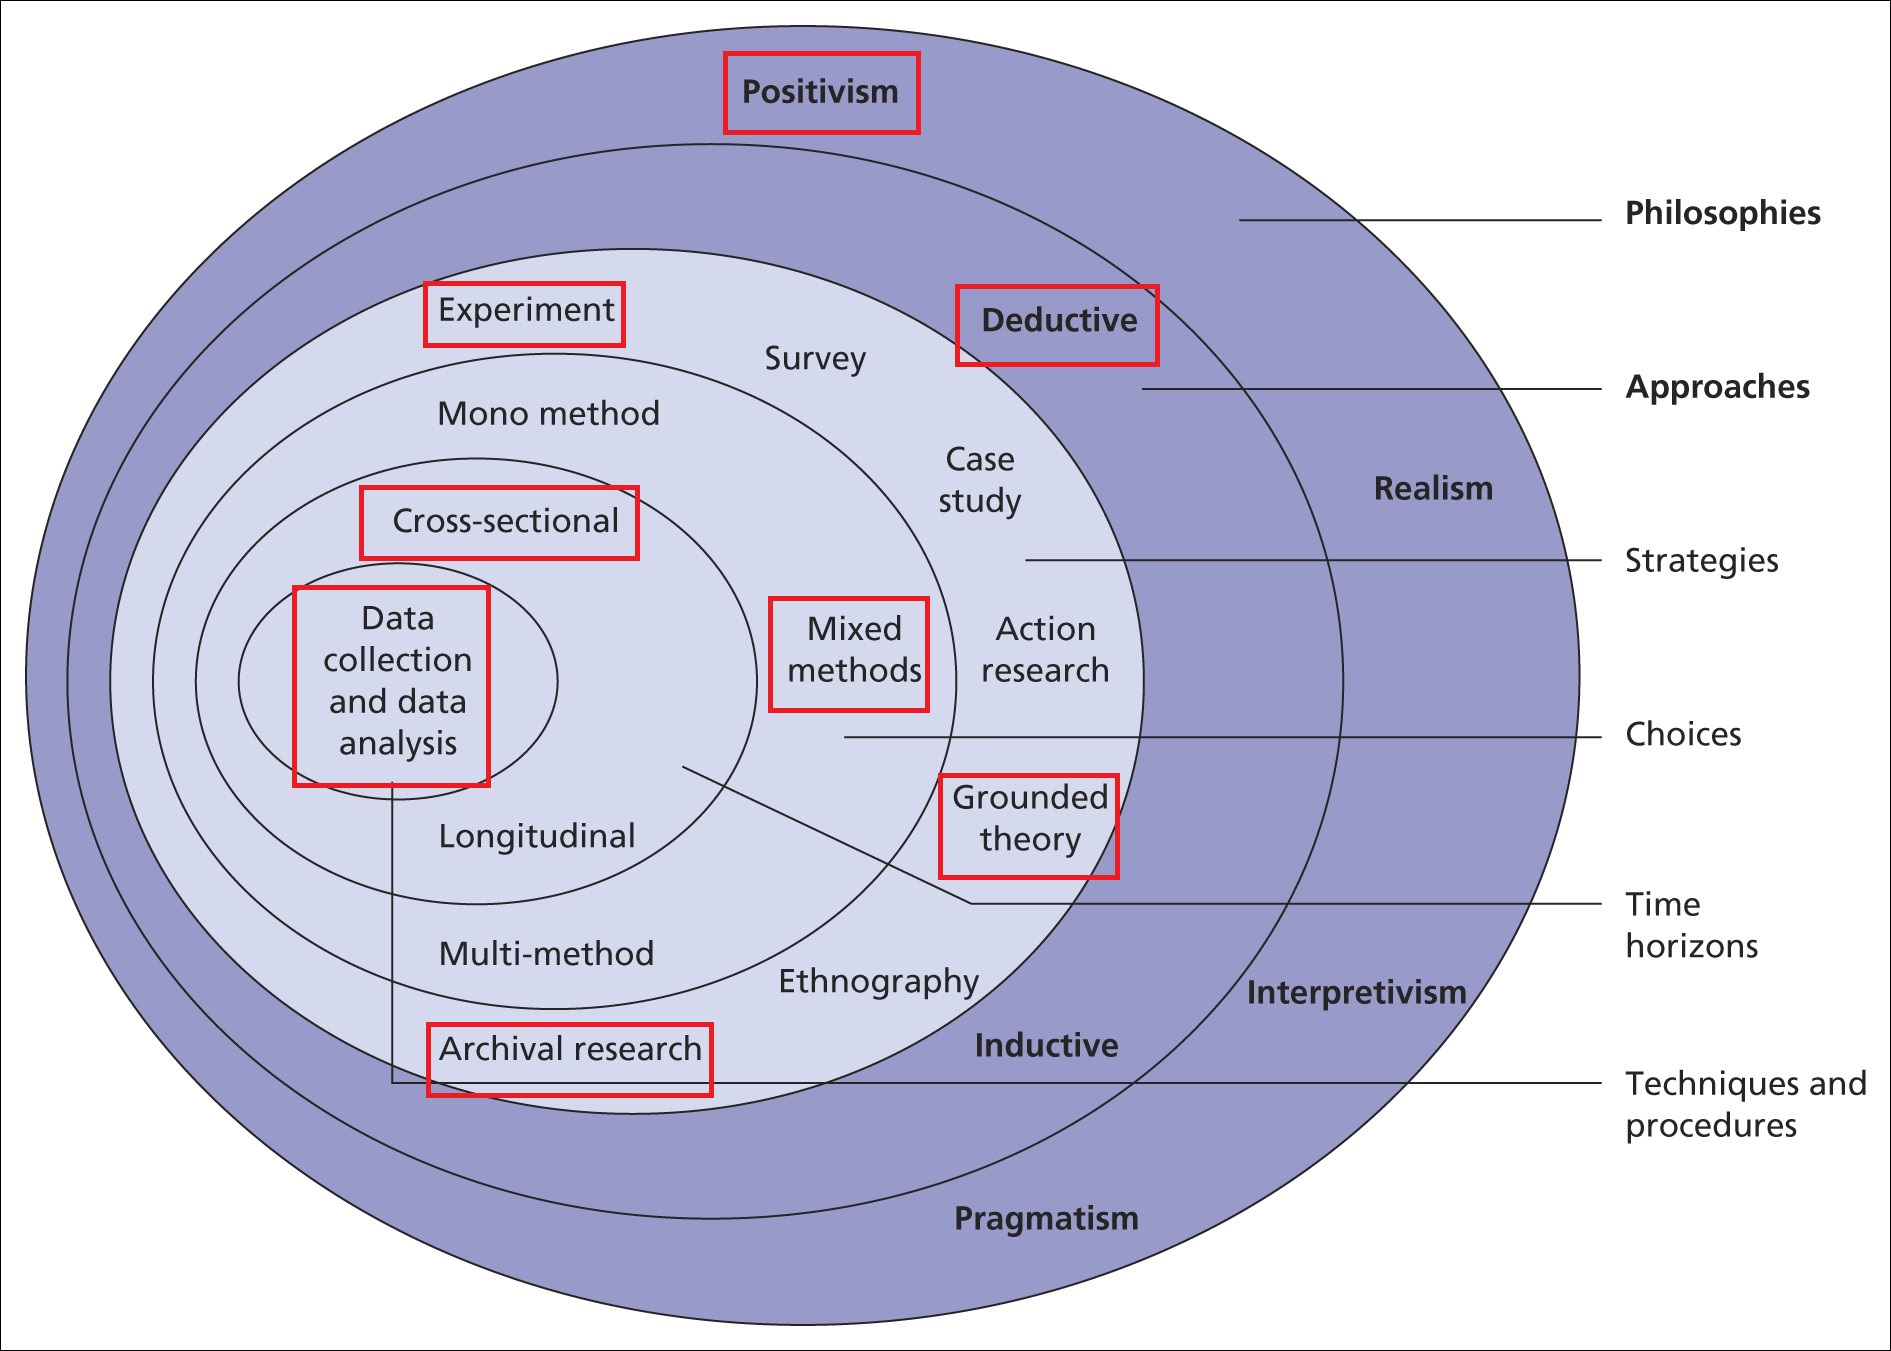
\includegraphics[scale=0.15]{Figures/Research-Onion.jpg}
\caption{Relevant research onion sections.\\Source: https://15writers.com/research-onion/}
\label{fig:Onion} 
\end{figure}

\end{spacing}

%=== END OF CHAPTER ONE ===
\newpage


